\documentclass[tikz,svgnames]{standalone}
\usepackage{wx672tikz}

\begin{document}
\begin{tikzpicture}
  \node (bg) [anchor=south west, inner sep=0] at (0,0) {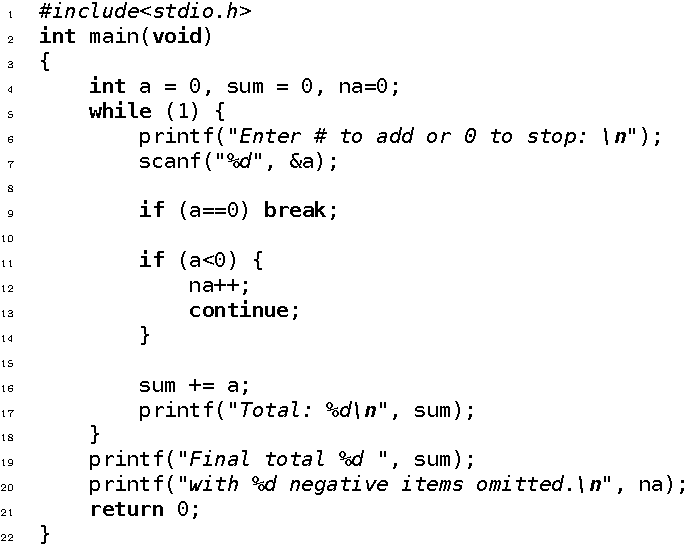
\includegraphics{bw/continue-c}};

  \begin{scope}[x={(bg.south east)},y={(bg.north west)}]% 
    %%% grid
    % \draw[help lines,xstep=.1,ystep=.1] (0,0) grid (1,1);%
    % \foreach \x in {0,1,...,9} { \node [xy,anchor=north] at (\x/10,0) {\x}; }% 
    % \foreach \y in {0,1,...,9} { \node [xy,anchor=east] at (0,\y/10) {\y};}% 

    \draw[->, opacity=.2,ultra thick,red] (.44,.59) to[bend left=40] (.15,.18);   % break
    \draw[->, opacity=.2,ultra thick,red] (.28,.43) to[bend left=75] (.2,.74); % continue
  \end{scope}
\end{tikzpicture}
\end{document}
%%% Local Variables:
%%% mode: latex
%%% TeX-master: t
%%% End:
